\documentclass[letterpaper,12pt]{article}
\pdfsuppresswarningpagegroup=1
\pdfoutput=1 % if your are submitting a pdflatex (i.e. if you have
             % images in pdf, png or jpg format)

\usepackage{jheppub} % for details on the use of the package, please
                     % see the JHEP-author-manual
\usepackage[utf8]{inputenc}
\usepackage[spanish,activeacute,es-nodecimaldot]{babel}

\usepackage{jheppub} %
\usepackage{amsmath}%
\usepackage{amsfonts}%
\usepackage{amscd}%
\usepackage{latexsym,amssymb} %\usepackage{pythonhighlight}
\usepackage[section]{placeins}
\usepackage{afterpage}%\usepackage{graphicx}
\usepackage[T1]{fontenc} % if needed
\usepackage{physics}
\usepackage{epigraph}
\usepackage{tcolorbox}%\usepackage{dsfont}
\usepackage{listings}
\usepackage{tikz-cd}


\title{{\boldmath{ Memoria Densamente Asociada}}
           }
\collaboration{Una perspectiva bio inspirada de redes neuronales \\}
%% %simple case: 2 authors, same institution
%% \author{A. Uthor}
%% \author{and A. Nother Author}
%% \affiliation{Institution,\\Address, Country}
%\vspace{30pt}
% more complex case: 4 authors, 3 institutions, 2 footnotes
\author[1]{Sergio Nieto}
%\author[c]{S. Econd Sergio,}
%\author[a,2]{T. Hird\note{Also at Some University.}}
%\author[a,2]{and Fourth}

% The "\note" macro will give a warning: "Ignoring empty anchor..."
% you can safely ignore it.

\affiliation{Facultad de Ciencias\note{Curso: Seminario de Matemáticas Aplicadas}, UNAM.}
%\affiliation[b]{Another University,\\different-address, Country}
%\affiliation[c]{A School for Advanced Studies,\\some-location, Country}

% e-mail addresses: one for each author, in the same order as the authors
\emailAdd{ssnieto@ciencias.unam.mx}
%\emailAdd{second@asas.edu}
%\emailAdd{third@one.univ}
%\emailAdd{fourth@one.univ}




\abstract{Abstract... \emph{some text}}



\begin{document}
\maketitle
\flushbottom

\section{Introducción}
\label{sec:intro}


Aprendizaje.\\

\parindent=0cm Memoria.\\

Este trabajo. \\

\section{Redes Neuronales}
\label{sec:nn}

 Una red neuronal artificial~\cite{dl} es un modelo matemático inspirado en redes neuronales biológicas. Consiste de un grupo entrelazado de nodos o neuronas artificiales individuales cuya estructura se escoge de acuerdo al problema que se enfrenta. \\

La estructura y funcionamiento del sistema nervioso central~\cite{neuro} tiene como parte constituyente a la neurona biológica que consiste en un cuerpo celular, el axón, las dendritas y las sinapsis. Estas últimas son las conexiones entre neuronas. El mecanismo sináptico es el que se busca mapear a un algoritmo analítico.\\

Una neurona artificial, ver figura~\ref{neuron}, se conoce también como \emph{perceptrón} y su forma básica es la siguiente:

\begin{equation}
  y(x_1, \dots, x_n) = f(w_1 x_1 + \dots w_n x_n + b)
\end{equation}

Donde cada $x_i$ se toma en cuenta individualmente por medio de un peso aprendido $w_i$. Esto nos permite construir un mapeo de $(x_1, \dots, x_n) = \bf{x} \in \mathbb{R}^n$ a la variable de salida $y$. La función $f$ se puede definir como una función de salto:

\begin{equation*}
f(s)=\begin{cases}
          0 \quad &\text{if} \, s \leq 0 \\
          1 \quad &\text{if} \, s > 0 \\
     \end{cases}
\end{equation*}

El valor $b$ conocido como \emph{bias o sesgo} permite aplicar la función $f$ a hiperplanos que no pasan por el origen. De esta forma el perceptrón, ver figura~\ref{perceptron}, es la composición de una transformación afín seguida de una función de salto que también se denomina como \emph{función de activación}. Esta no necesariamente es una función de salto y se elige según el problema que se esta tratando de resolver. \\

\begin{figure}
\begin{center}
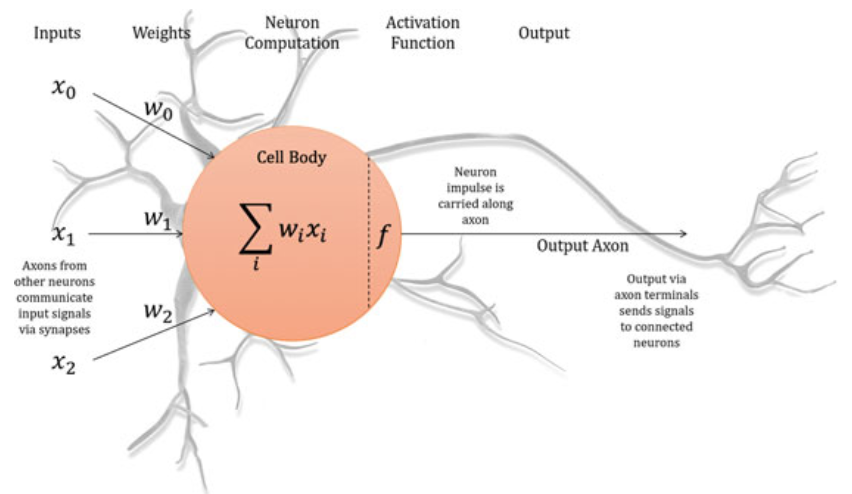
\includegraphics[height=55mm]{neuron.PNG}
\caption{\small{Neurona artificial. }}
\label{neuron}
\end{center}
\end{figure}
%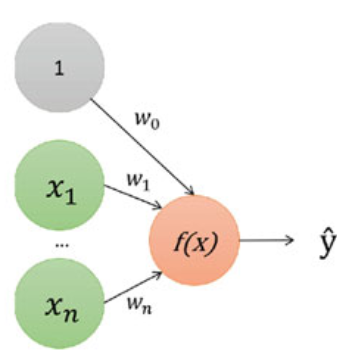
\includegraphics[width=.4\textwidth,origin=c]{perceptron.PNG}
\begin{figure}
\begin{center}
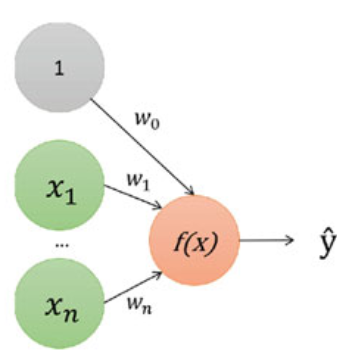
\includegraphics[height=50mm]{perceptron.PNG}
\caption{\small{Esquema de un Perceptrón. }}
\label{perceptron}
\end{center}
\end{figure}

\section{Redes de Memoria Asociada}
\label{sec:hop}

For internal references use label-refs: see section~\ref{sec:intro}.
Bibliographic citations can be done with cite: refs.~\cite{a,b0,c}.
When possible, align equations on the equal sign. The package
\texttt{amsmath} is already loaded. See \eqref{eq:x}.
\begin{equation}
\label{eq:x}
\begin{split}
x &= 1 \,,
\qquad
y = 2 \,,
\\
z &= 3 \,.
\end{split}
\end{equation}
Also, watch out for the punctuation at the end of the equations.


\begin{equation*}
g(x)=\begin{cases}
          x \quad &\text{if} \, x \in \mathbb{Q} \\
          -x \quad &\text{if} \, x \notin \mathbb{Q} \\
     \end{cases}
\end{equation*}

If you want some equations without the tag (number), please use the available
starred-environments. For example:
\begin{equation*}
x = 1
\end{equation*}

The amsmath package has many features. For example, you can use use
\texttt{subequations} environment:
\begin{subequations}\label{eq:y}
\begin{align}
\label{eq:y:1}
a & = 1
\\
\label{eq:y:2}
b & = 2
\end{align}
and it will continue to operate across the text also.
\begin{equation}
\label{eq:y:3}
c = 3
\end{equation}
\end{subequations}
The references will work as you'd expect: \eqref{eq:y:1},
\eqref{eq:y:2} and \eqref{eq:y:3} are all part of \eqref{eq:y}.

A similar solution is available for figures via the \texttt{subfigure}
package (not loaded by default and not shown here).
All figures and tables should be referenced in the text and should be
placed at the top of the page where they are first cited or in
subsequent pages. Positioning them in the source file
after the paragraph where you first reference them usually yield good
results. See figure~\ref{fig:i} and table~\ref{tab:i}.

\begin{figure}[tbp]
\centering % \begin{center}/\end{center} takes some additional vertical space
\includegraphics[width=.45\textwidth,trim=0 380 0 200,clip]{img1.pdf}
\hfill
\includegraphics[width=.45\textwidth,origin=c,angle=180]{img2.pdf}
% "\includegraphics" is very powerful; the graphicx package is already loaded
\caption{\label{fig:i} Always give a caption.}
\end{figure}

\begin{table}[tbp]
\centering
\begin{tabular}{|lr|c|}
\hline
x&y&x and y\\
\hline
a & b & a and b\\
1 & 2 & 1 and 2\\
$\alpha$ & $\beta$ & $\alpha$ and $\beta$\\
\hline
\end{tabular}
\caption{\label{tab:i} We prefer to have borders around the tables.}
\end{table}

We discourage the use of inline figures (wrapfigure), as they may be
difficult to position if the page layout changes.

We suggest not to abbreviate: ``section'', ``appendix'', ``figure''
and ``table'', but ``eq.'' and ``ref.'' are welcome. Also, please do
not use \texttt{\textbackslash emph} or \texttt{\textbackslash it} for
latin abbreviaitons: i.e., et al., e.g., vs., etc.



\section{Sections}
\subsection{And subsequent}
\subsubsection{Sub-sections}
\paragraph{Up to paragraphs.} We find that having more levels usually
reduces the clarity of the article. Also, we strongly discourage the
use of non-numbered sections (e.g.~\texttt{\textbackslash
  subsubsection*}).  Please also see the use of
``\texttt{\textbackslash texorpdfstring\{\}\{\}}'' to avoid warnings
from the hyperref package when you have math in the section titles



\appendix
\section{Some title}
Please always give a title also for appendices.





\acknowledgments

This is the most common positions for acknowledgments. A macro is
available to maintain the same layout and spelling of the heading.

\paragraph{Note added.} This is also a good position for notes added
after the paper has been written.


%articles: author(s), title, journal name, volume, year, page number, arXiv-number. Addi- tional information (erratum, addendum) can be specified too.

\begin{thebibliography}{99}

\bibitem{dl}
Goodfellow I., Bengio Y., Courville A., \emph{Deep Learning}, MIT Press, 2016.

\bibitem{neuro}
Bear M., Connors B., Paradiso M., \emph{Neuroscience. Exploring the Brain}, Wolters Kluwer, 2015.

\bibitem{a}
Hopfield J. J., \emph{Neural networks and physical systems with emergent collective computational abilities}, \emph{Proc. Natl. Acad. Sci. USA} {\bf 79} (1982) pp. 2554-2558.

\bibitem{b0}
Krotov D., Hopfield J. J., \emph{Dense associative memory for pattern recognition}, \emph{Advances in neural information processing systems} {\bf 29} (2016) pp.1172-1180.

\bibitem{b1}
Krotov D., Hopfield J. J., \emph{Dense associative memory is robust for adversarial inputs}, \emph{Neural Computation} {\bf 30} (2018) pp.3151-3167.

\bibitem{b2}
Krotov D., Hopfield J. J., \emph{Large associative memory problem in neurobiology and machine learning}, arxiv:2008.06996v3.

\bibitem{c}
Ramsauer H., Schafl B., Lehner J., Seidl P., Widrich M., Gruber L., Holzleitner M., Pavlovi'c M., Kjetil Sandve G., Greiff V., Kreil D., Kopp M., Klambauer G., Brandstetter J., Hochreiter S., \emph{Hopfield Networks is All You Need}, arxiv:2008.02217.

\bibitem{d}
Roy S., Chakraborty U., \emph{Introduction to Soft Computing. Neuro-fuzzy and Genetic Algorithms}, Pearson India, 2013.

\bibitem{e}
Gabbiani F., Cox F.J., \emph{Mathematics for Neuroscientists}, Academic Press, 2010.

\end{thebibliography}
\end{document}
